\documentclass[a4paper,12pt,twoside,openany]{report}
%
% Wzorzec pracy dyplomowej
% J. Starzynski (jstar@iem.pw.edu.pl) na podstawie pracy dyplomowej
% mgr. inż. Błażeja Wincenciaka
% Wersja 0.1 - 8 października 2016
%
\usepackage{polski}
\usepackage{helvet}
\usepackage[T1]{fontenc}
\usepackage{anyfontsize}
\usepackage[utf8]{inputenc}
\usepackage[pdftex]{graphicx}
\usepackage{tabularx}
\usepackage{array}
\usepackage[polish]{babel}
\usepackage{subfigure}
\usepackage{amsfonts}
\usepackage{algorithmicx}
\usepackage{algpseudocode}
\usepackage{algorithm}
\usepackage{verbatim}
\usepackage{indentfirst}
\usepackage[pdftex]{hyperref}
\usepackage{bm}
\usepackage{amsmath}

% rozmaite polecenia pomocnicze
% gdzie rysunki?
\graphicspath{ {rys/} }
% oznaczenie rzeczy do zrobienia/poprawienia
\newcommand{\TODO}{\textbf{TODO}}
\newcommand*\NewPage{\newpage\null\thispagestyle{empty}\newpage}



% wyroznienie slow kluczowych
\newcommand{\tech}{\texttt}

% na oprawe (1.0cm - 0.7cm)*2 = 0.6cm
% na oprawe (1.1cm - 0.7cm)*2 = 0.8cm
%  oddsidemargin lewy margines na nieparzystych stronach
% evensidemargin lewy margines na parzystych stronach
\def\oprawa{1.05cm}
\addtolength{\oddsidemargin}{\oprawa}
\addtolength{\evensidemargin}{-\oprawa}

% table span multirows
\usepackage{multirow}
\usepackage{enumitem}    % enumitem.pdf
\setlist{listparindent=\parindent, parsep=\parskip} % potrzebuje enumitem

%%%%%%%%%%%%%%% Dodatkowe Pakiety %%%%%%%%%%%%%%%%%
\usepackage{prmag2017}   % definiuje komendy opieku,nrindeksu, rodzaj pracy, ...
\usepackage{xspace}

%%%%%%%%%%%%%%% Strona Tytułowa %%%%%%%%%%%%%%%%%
% To trzeba wypelnic swoimi danymi
\title{Aplikacja do rozpoznawania emocji w sygnale mowy}

% autor
\author{Wojciech Decker}
\nrindeksu{252545}


\opiekun{dr inż. Andrzej Majkowski}
\konsultant{prof. Dzielny Konsultant}  % opcjonalnie
\terminwykonania{1 września 2017} % data na oświadczeniu o samodzielności
\rok{2017}


% Podziekowanie - opcjonalne
\podziekowania{\noindent
{\Large Podziękowania}
\bigskip

Dziękujemy bardzo serdecznie wszystkim, a w szczególności Rodzinom i~Unii Europejskiej...

\bigskip

{\raggedleft
Zdolny Student i Pracowity Kolega

}

}

% To sa domyslne wartosci
% - mozna je zmienic, jesli praca jest pisana gdzie indziej niz w ZETiIS
% - mozna je wyrzucic jesli praca jest pisana w ZETiIS
%\miasto{Warszawa}
%\uczelnia{POLITECHNIKA WARSZAWSKA}
%\wydzial{WYDZIAŁ ELEKTRYCZNY}
%\instytut{INSTYTUT ELEKTROTECHNIKI TEORETYCZNEJ\linebreak[1] I~SYSTEMÓW INFORMACYJNO-POMIAROWYCH}
\zaklad{ZAKŁAD SYSTEMÓW INFORMACYJNO POMIAROWYCH}
%\kierunekstudiow{INFORMATYKA}

% domyslnie praca jest inzynierska, ale po odkomentowaniu ponizszej linii zrobi sie magisterska
\pracamagisterska
%%% koniec od P.W

\opinie{%
	\newpage
\begin{center}
 {\large\bf  Opinia} \\
o pracy dyplomowej magisterskiej wykonanej przez dyplomanta\\
{\bf Zdolnego Studenta i Pracowitego Kolegę} \\
 Wydział Elektryczny, kierunek Informatyka,  Politechnika Warszawska\\
Temat pracy\\
\textit{\bf
TYTUŁ PRACY DYPLOMOWEJ
}\\
\end{center}
\medskip
\noindent
Promotor: {\bf dr inż. Miły Opiekun}\\
Ocena pracy dyplomowej: {\bf bardzo dobry}

\medskip

\centerline{\bf Treść opinii}
   Celem pracy dyplomowej panów dolnego Studenta i Pracowitego Kolegi  było
opracowanie systemu pozwalającego symulować  i opartego o oprogramowanie o
otwartych źródłach (ang. Open Source). Jak piszą Dyplomanci, starali się opracować
system, który łatwo będzie dostosować do zmieniających się dynamicznie wymagań,
będzie miał niewielkie wymagania sprzętowe i umożliwiał dalszą łatwą rozbudowę oraz
dostosowanie go do potrzeb.
Przedstawiona do recenzji praca składa się z krótkiego wstępu jasno i
wyczerpująco opisującego oraz uzasadniającego cel pracy, trzech rozdziałów (2-4)
zawierających opis istniejących podobnych
rozwiązań, komponentów rozpatrywanychjako kandydaci do
tworzonego systemu i wreszcie zagadnień wydajności wirtualnych
rozwiązań. Piąty rozdział to opis przygotowanego przez
Dyplomantów środowiska obejmujący opis konfiguracji
środowiska oraz przykładowe ćwiczenia laboratoryjne. Ostatni
rozdział pracy to opis możliwości dalszego
rozwoju projektu. W ramach przygotowania pracy Dyplomanci zebrali i przedstawili w
bardzo przejrzysty sposób duży zasób informacji, co świadczy o dobrej orientacji
w nowoczesnej i ciągle intensywnie rozwijanej tematyce stanowiącej
zakres pracy i o umiejętności przejrzystego przedstawienia tych
wyników. Praca zawiera dwa dodatki, z których pierwszy obejmuje wyniki
eksperymentów i badań nad wydajnością, a drugi to źródła
skryptów budujących środowisko.

 Dyplomanci dość
dobrze zrealizowali postawione przed nimi zadanie,
wykazali się więc umiejętnością zastosowania w praktyce wiedzy
przedstawionej w rozdziałach 2-4.  Uważam, że cele postawione w założeniach pracy zostały pomyślnie
zrealizowane. Proponuję ocenę bardzo dobrą (5).

\vskip 1cm
{
\raggedleft
(data, podpis)\kern1cm

}
	\newpage
	\newpage
\begin{center}
 {\large\bf  Recenzja } \\
pracy dyplomowej magisterskiej wykonanej przez dyplomanta\\
{\bf Zdolnego Studenta i Pracowitego Kolegę} \\
 Wydział Elektryczny, kierunek Informatyka,  Politechnika Warszawska\\
Temat pracy\\
\textit{\bf
TYTUŁ PRACY DYPLOMOWEJ
}\\
\end{center}
\medskip
\noindent
Recenzent: {\bf prof. nzw. dr hab. inż. Jan Surowy}\\
Ocena pracy dyplomowej: {\bf bardzo dobry}
\medskip


\centerline{\bf Treść recenzji}
   Celem pracy dyplomowej panów dolnego Studenta i Pracowitego Kolegi  było
opracowanie systemu pozwalającego symulować  i opartego o oprogramowanie o
otwartych źródłach (ang. Open Source). Jak piszą Dyplomanci, starali się opracować
system, który łatwo będzie dostosować do zmieniających się dynamicznie wymagań,
będzie miał niewielkie wymagania sprzętowe i umożliwiał dalszą łatwą rozbudowę oraz
dostosowanie go do potrzeb.
Przedstawiona do recenzji praca składa się z krótkiego wstępu jasno i
wyczerpująco opisującego oraz uzasadniającego cel pracy, trzech rozdziałów (2-4)
zawierających bardzo solidny i przejrzysty opis: istniejących podobnych
rozwiązań (rozdz. 2), komponentów rozpatrywanychjako kandydaci do
tworzonego systemu (rozdz. 3) i wreszcie zagadnień wydajności wirtualnych
rozwiązań, zwłaszcza w kontekście współpracy  kilku elementów
 sieci (rozdział 4). Piąty rozdział to opis przygotowanego przez
Dyplomantów środowiska obejmujący opis konfiguracji
środowiska oraz przykładowe ćwiczenia laboratoryjne (5 ćwiczeń). Ostatni, szósty
rozdział pracy to krótkie zakończenie, które wylicza także możliwości dalszego
rozwoju projektu. W ramach przygotowania pracy Dyplomanci zebrali i przedstawili w
bardzo przejrzysty sposób duży zasób informacji o narzędziach, Rozdziały 2, 3 i 4 świadczą o dobrej orientacji
w nowoczesnej i ciągle intensywnie rozwijanej tematyce stanowiącej
zakres pracy i o umiejętności syntetycznego, przejrzystego przedstawienia tych
wyników. Drobne  mankamenty tej części pracy to zbyt skrótowe omawianie
niektórych zagadnień technicznych, zakładające dużą początkową wiedzę czytelnika
i dość niestaranne podejście do powołań na źródła.
Utrudnia to w pewnym stopniu czytanie pracy i zmniejsza jej wartość dydaktyczną
(a ta zdaje się być jednym z celów Autorów), ale jest zrekompensowane zawartością
merytoryczną. Praca zawiera dwa dodatki, z których pierwszy obejmuje wyniki
eksperymentów i badań nad wydajnością, a drugi to źródła
skryptów budujących środowisko. Praca
zawiera niestety dość dużą liczbę drobnych błędów redakcyjnych, ale nie wpływają
one w sposób istotny na na jej czytelność i wartość. W całej pracy przewijają
się samodzielne, zdecydowane wnioski Autorów, które są wynikiem własnych i
oryginalnych badań.  Rozdział 5 i dodatki pracy przekonują mnie, że Dyplomanci dość
dobrze zrealizowali postawione przed nimi zadanie. Pozwala to stwierdzić, że
wykazali się więc także umiejętnością zastosowania w praktyce wiedzy
przedstawionej w rozdziałach 2-4. Kończący pracę rozdział szósty świadczy o
dużym (ale moim zdaniem uzasadnionym) poczuciu własnej wartości i jest
świadectwem własnego, oryginalnego spojrzenia na tematykę przedstawioną w pracy
dyplomowej. Uważam, że cele postawione w założeniach pracy zostały pomyślnie
zrealizowane. Proponuję ocenę bardzo dobrą (5).

\vskip 1cm
{
\raggedleft
(data, podpis)\kern1cm

}
}

\streszczenia{
	\newpage
\begin{center}
\large \bf
TYTUŁ PRACY DYPLOMOWEJ
\end{center}

\section*{Streszczenie}
Praca składa się z krótkiego wstępu jasno i
wyczerpująco opisującego oraz uzasadniającego cel pracy, trzech rozdziałów (2-4)
zawierających opis istniejących podobnych
rozwiązań, komponentów rozpatrywanychjako kandydaci do
tworzonego systemu i wreszcie zagadnień wydajności wirtualnych
rozwiązań. Piąty rozdział to opis  środowiska obejmujący opis konfiguracji
środowiska oraz przykładowe ćwiczenia laboratoryjne. Ostatni
rozdział pracy to opis możliwości dalszego
rozwoju projektu. 

\bigskip
{\noindent\bf Słowa kluczowe:} praca dyplomowa, LaTeX, jakość

\vskip 2cm


\begin{center}
\large \bf
THESIS TITLE
\end{center}

\section*{Abstract}
This thesis presents a novel way of using a novel algorithm to solve complex
problems of filter design. In the first chapter the fundamentals of filter design
are presented. The second chapter describes an original algorithm invented by the
authors. Is is based on evolution strategy, but uses an original method of filter
description similar to artificial neural network. In the third chapter the implementation
of the algorithm in C programming language is presented. The fifth chapter contains results
of tests which prove high efficiency and enormous accuracy of the program. Finally some
posibilities of further development of the invented algoriths are proposed.

\bigskip
{\noindent\bf Keywords:} thesis, LaTeX, quality

\vfill
}
\newcommand{\ang}[1]{\textit{(ang. #1)}}
\newcommand{\MATLAB}{\textsc{Matlab}\xspace}

\begin{document}
\maketitle
%-----------------
% Wstęp
%-----------------
\chapter{Wstęp}
\label{ch:wstep}
% krótka definicja emocji
Emocje to stany ludzkiego umysłu.
Powstają w odpowiedzi na zdarzenie, są ukierunkowane i krótkotrwałe.
Różnią się intensywnością i zabarwieniem.
Wpływają na interpretację bodźców z otoczenia,
myśli a w konsekwencji mają istotny wpływ na zachowanie i reakcje.

% informacje zakodowane w mowie
Mowa jest nośnikiem informacji wykorzystywanym w komunikacji międzyludzkiej,
oraz pomiędzy człowiekiem i komputerem \ang{Human-Computer Interaction}.
Komunikat głosowy składa się z treści językowej,
którą można zapisać w formie tekstu,
oraz akustycznej, która również opisuje wypowiedź takie jak:
drżący ze strachu głos, czy ciężki oddech świadczący o gniewie.

% Zastosowanie maszynowego rozpoznawania emocji
Rozpoznawanie emocji mówcy jest istotne w aplikacjach wykorzystujących mowę w komunikacji człowiek-maszyna.
Zwłaszcza, jeśli odpowiedź systemu jest uzależniona od nastroju człowieka.
Klasyfikacja emocji wypowiedzi jest wykorzystywana w terapiach,
gdzie terapeuta wspiera się maszyną w odczytywaniu emocji pacjenta.
Systemy tłumaczenia maszynowego mowy mogą wykorzystać informacje mówiące o kontekście wypowiedzi i stanie mówcy.
Telefoniczne centra obsługi klienta \ang{call center} rozpoznają stan klienta,
oraz jego reakcję na ofertę prezentowaną przez konsultanta.

% Jaki jest cel?
Celem pracy jest przybliżenie tematyki komputerowego rozpoznawania mowy,
przegląd wykorzystywanych narzędzi, oraz ocena znanych rozwiązań.
Produktem końcowym będzie aplikacja komputerowa rozpoznająca emocje w sygnale mowy.
W trakcje tworzenia pracy zostanie dokonana analiza znanych rozwiązań tego zagadnienia.
Następnie zostanie opracowany schemat aplikacji, bazujący na poprzednich badaniach,
pozwalający stworzyć aplikację w warunkach tworzenia pracy magisterskiej.
Kolejnym etapem będzie implementacja aplikacji w środowisku MATLAB.
Na zakończenie zostaną przeprowadzone testy aplikacji,
analiza wyników i prezentacja wniosków.

% roboczo
Jakie współczynniki można liczyć? 
Jak przetworzyć dane, żeby otrzymać lepsze wyniki?
Jakie przetwarzanie jest wymagane?
\NewPage
\chapter{Aplikacja klasyfikująca emocje}
\section{Opis bazy danych}
\TODO{sposób katalogowania}
W pracy wykorzystano bazę danych emocji w mowie powstały w Akademii Górniczo-Hutniczej w Krakowie.
Nagrania zawierają pięć emocji podstawowych: radość, smutek, złość, strach, zdziwienie.
Ponadto zostały nagrane wypowiedzi w tonie neutralnym jako punkt odniesienia i ironicznym, jako emocja złożona.
W nagraniu wzięło udział 6 mężczyzn i 6 kobiet od 20 do 30 lat. 
Mówcy byli zarówno profesjonalnymi aktorami jak i amatorami, czy wolontariuszami.
Baza została zrealizowana jako baza danych emocji odgrywanych. 

Nagrano 4 typy wypowiedzi.
\begin{description}
	\item [Zdania] będące sekwencją 46 prostych wypowiedzi często wykorzystywanych w życiu codziennym 
		np. ,,Dzień dobry'', ,,Witam serdecznie''. 
	\item [Polecenia]  np. ,,Nowy'', ,,Otwórz''. 
		Jest to głosowa reprezentacja standardowych komend wykorzystywanych w komunikacji człowieka z komputerem.
	\item [Cyfry] od 0 do 9.
	\item [Tekst] czyli fragment artykułu. 
		Lity tekst będący spójnym logicznie ciągiem zdań, lecz wyrwanym z kontekstu.
\end{description}
Dla każdego z 6 mówców zarejestrowano każdy typ wypowiedzi we wszystkich stanach emocjonalnych.

Baza danych składa się z opisu, oraz wypowiedzi posegregowanych w katalogach oznaczających odgrywaną emocję.
Nazwy plików wskazują na mówcę, emocję oraz typ wypowiedzi.
Nagrania zostały zapisane w formie plików WAV przy częstotliwości próbkowania 44100Hz i rozdzielczości 16 bitów. ~\cite{Igras2009}.

Nagrania nie zostały poddane przetwarzaniu wstępnemu. 
Różnią się poziomem głośności.
Pojedyncze nagrania wyglądają na ustandaryzowane, ale stanowią wyjątek.
Dokładna historia nagrań nie jest znana, ich stan jest niejednolity.
Brak jest informacji o operacjach wykonywanych na nagraniach.
Stan nagrań jest niejednorodny i nieznany.
\begin{figure}[h]
	\centering
	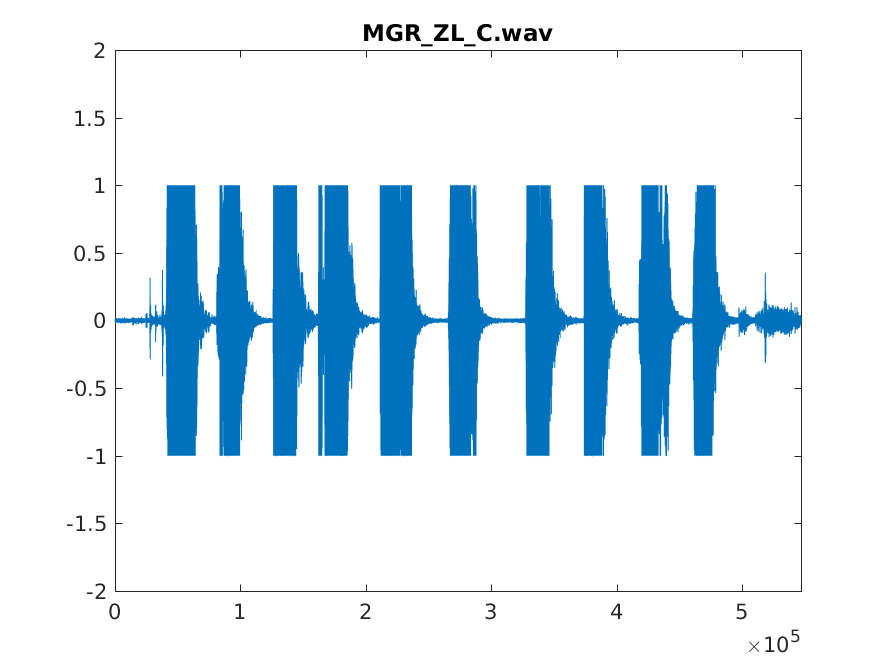
\includegraphics[width=\textwidth]{MGR_ZL_C-plot}
	\caption{Przykład ustandaryzowanego sygnału}
\end{figure}
\begin{figure}[h]
	\centering
	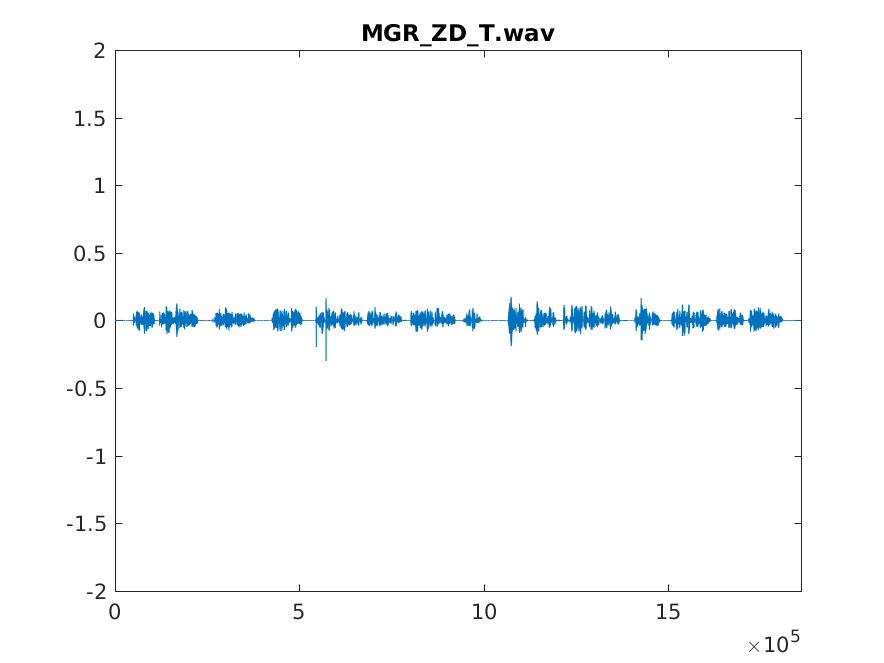
\includegraphics[width=\textwidth]{MGR_ZD_T-plot}
	\caption{Przykład nie ustandaryzowanego sygnału}
\end{figure}

Zapis wypowiedzi został ustandaryzowany w celu zniwelowania różnic wynikających z głośności nagrania.
\section{Przetwarzanie wstępne}
\TODO{od czytania pliku z dysku, do rozpoczęcia ekstrakcji cech}
\NewPage
\NewPage
\section{Ekstrakcja cech}
\subsection{Cechy bazowe}
\subsubsection{MFCC}
\NewPage
\NewPage
\subsubsection{Energia}
\subsubsection{Liczba przejść przez zero}
\subsubsection{Energia entropii}
\NewPage
\subsubsection{SSC}
\NewPage
\NewPage
\subsection{Opis statystyczny}
\TODO{Opisać  'minmax', 'mean', 'variance', 'skewness', 'kurtosis'}
\NewPage
\NewPage
\NewPage
\section{Selekcja cech}
\subsection{SFS}
\NewPage
\NewPage
\NewPage
\subsection{PCA}
\NewPage
\NewPage
\NewPage
\section{Klasyfikacja}
\subsection{Klasyfikator Najbliższych Sąsiadów}
Klasyfikator najbliższych sąsiadów pozwala szybko otrzymać rezultaty. 
Jest prosty w działaniu i implementacji.
Otrzymane rezultaty mogą nie być zadowalające w bardziej złożonych zagadnieniach.
Zasada działania w uproszczeniu sprowadza się do reprezentacji obserwacji za pomocą wektorów cech.
Obliczane są odległości pomiędzy wektorami. \cite{Du2013}
Klasa jest przypisywana na podstawie klasy najbliższej, sąsiedniej obserwacji.
Klasyfikator jest podatny na ilość cech branych pod uwagę w czasie klasyfikacji.
Redukcja liczby parametrów, uwzględniająca usunięcie cech silnie skorelowanych i słabo różnicujących znacząco podnosi wydajność i skuteczność klasyfikatora.

Metoda klasyfikuje obserwacje biorąc pod uwagę najbliższą obserwację ze zbioru uczącego.
Obserwacje ze zbioru uczącego rozmieszczone są w wielowymiarowej przestrzeni cech.
Przestrzeń ta jest podzielona na strefy odpowiadające klasom.
Obserwacja znajdująca się w danej strefie zostaje przypisana do klasy do której ta strefa należy.
Podział na strefy odbywa się w czasie fazy uczenia klasyfikatora.
Kształt i klasa strefy zależy od odległości obserwacji ze zbioru uczącego.
Punkt w przestrzeni przypisany zostaje do klasy, jeżeli w jego najbliższym sąsiedztwie zostanie znalezionych $k$ sąsiadów należących do tej klasy.
Klasyfikatorowi należy zdefiniować liczbę $k$ - liczbę wymaganych sąsiadów klasy, pozwalającą określić klasę badanej obserwacji, 
oraz funkcję liczącą dystans pomiędzy dwoma wektorami. Najczęściej jest to norma euklidesowa. \cite{Martin2011}

\begin{algorithm}
	\caption{Klasyfikator Najbliższych sąsiadów}
	\begin{algorithmic}[1]
		\Procedure {kNN}{$T$, $k$, $dist$, $o$}
		\State $D \leftarrow []$
		\ForAll {$t \in T$}
		\State $D(t) \leftarrow dist(t, o)$
		\EndFor
		\State $S \leftarrow sort(D, T)$ \Comment obserwacje posortowane względem odległości
		\State $selectedClass \leftarrow 0$
		\State $counter \leftarrow []$ \Comment licznik najbliższych sąsiadów z klasy
		\Repeat
		\ForAll {$s \in S$}
		\State $counter(class(s))++$
		\EndFor
		\Until{$\neg selectedClass$}
		\EndProcedure
	\end{algorithmic}
\end{algorithm}

Dane wejściowe muszą być znormalizowane. 
W przeciwnym razie cechy o bezwzględnie wyższych wartościach będą miały większy wpływ na klasyfikację,
bez rozróżnienia ich zdolności różnicowania zbioru.
Algorytm jest wrażliwy na liczbę cech - wymiarów przestrzeni w której umieszczana jest obserwacja.
Każda cecha wprowadza wymiar równoważny z pozostałymi wymiarami. 
Nie jest brana pod uwagę korelacja cech, ani ich zdolność różnicowania obserwacji.
Dla klasyfikowanej obserwacji obliczany jest dystans pomiędzy nią,
a każdą obserwacją ze zbiory testowego, uwzględniająca wszystkie wymiary.
Prowadzi to do znacznego wzrostu złożoności obliczeniowej klasyfikacji, dla większej liczby cech, czy zbiorów danych uczących.

Istnieją modyfikacje klasyfikatora najbliższych sąsiadów redukujące wymienione wady. 
Opisana została klasyczna wersja algorytmu.

\subsection{Maszyny Wektorów Wspierających}

Maszyny Wektorów Wspierających \ang{Support Vector Machine} wykorzystywany jest do klasyfikacji obserwacji w uczeniu maszynowym.
Należy do grupy modeli uczonych w sposób nadzorowany. 
Uczenie odbywa się przez zadanie zbioru danych testowych, 
każda obserwacja jest oznaczona jako należąca do jednej z dwóch klas.
Algorytm uczący SVM tworzy model rozróżniający obserwacje obydwu klas.
Jako rezultat powstaje klasyfikator binarny, nie probabilistyczny. 

Model powstaje przez rozmieszczenie obserwacji w przestrzeni wielowymiarowej.
Każda obserwacja zostaje umieszczona w $n$-wymiarowej przestrzeni cech i reprezentowana jest przez wektor
zaczynający się w początku układu współrzędnych, a kończący się w punkcie określającym obserwację. 
Hiperpłaszczyzna \ang{hyperplane} jest $n-1$ wymiarowa i zgodnie z definicją rozdziela przestrzeń na dwie części.
Poszukiwana hiperpłaszczyzna powinna być hiperpłaszczyzną optymalną \ang{optimal hyperplane}, 
to czyli znajdować się w jak największej odległości od najbliższych obserwacji należących do różnych klas.
\cite{Cortes1995}

Biorąc przestrzeń dwuwymiarową, możemy ją rozmieścić na płaszczyźnie. 
Na płaszczyźnie tej kładziemy dowolną prostą. 
Prosta ta dzieli płaszczyznę na dwie części.
Prosta jest więc hiperpłaszczyzną przestrzeni dwuwymiarowej.
Analogicznie sytuacja przestawia się w przestrzeni trójwymiarowej.
Może ją przeciąć dowolna płaszczyzna.
Płaszczyzna dzieli przestrzeń trójwymiarową na dwie części, jest więc jej hiperpłaszczyzną.

Sposób tworzenia klasyfikatora SVM przedstawia się następująco.
Obserwacje $x_i$ rozmieszczone są w $n$-wymiarowej przestrzeni cech, gdzie $x_i \in R^n$.
Klasy $y_i$ są oznaczone jako $-1$ i $+1$, gdzie $y_i \in \{-1, +1\}$, co można zapisać jako:
\begin{equation}
	(\bm{x_1},y_1), ..., (\bm{x_i}, y_i), \textrm{ gdzie } y_i \in \{-1, +1\}
\end{equation}

Obserwacje są liniowo separowalne, jeżeli istnieje wektor $\bm{w}$ i taki skalar $b$, że nierówności
\begin{gather}
	\bm{w} \cdot \bm{x_i} + b \geq 1 \textrm{ jeśli } y_i = 1\\
	\bm{w} \cdot \bm{x_i} + b \leq 1 \textrm{ jeśli } y_i = -1,
\end{gather}
są prawdziwe dla wszystkich obserwacji w zbiorze.
\cite{Cortes1995}
Powyższy układ nierówności można zapisać w postaci:
\begin{equation}
	y_i(\bm{w} \cdot \bm{x_i} + b) \geq 1
\end{equation}
Hiperpłaszczyzna optymalna 
\begin{equation}
	\bm{w_0} \cdot \bm{x_i}  + b_0 = 0
\end{equation}

istnieje w przypadku, kiedy rozdziela zbiór treningowy z zachowaniem największej możliwej odległości od obserwacji obydwu klas.
Odległość pomiędzy obserwacjami a hiperpłaszczyzną definiuje się następująco:
\begin{equation}
	\rho(\bm{w}, b) = \min\limits_{\{x:y=1\}} \frac{\bm{x} \cdot \bm{w}} {|\bm{w}|} - \max\limits_{\{x:y=-1\}}  \frac{\bm{x} \cdot \bm{w}} {|\bm{w}|} 
\end{equation}
czyli rzut skalarny \ang{scalar projection} wektora obserwacji $\bm{x}$ na wektor jednostkowy $\hat{\bm{w}} = \frac{\bm{w}}{|\bm{w}|}$
obrazujący położenie płaszczyzny.
Wartość rzutu skalarnego jest odległością obserwacji od hiperpłaszczyzny. 
Różnica najmniejszej odległości pomiędzy hiperpłaszczyzną, a obserwacją należącą do klasy $y=1$,
oraz największej odległości pomiędzy hiperpłaszczyzną, a obserwacją należącą do klasy $y=-1$ 
powinna być jak największa.
Obserwacje znajdujące się w najmniejszej odległości od hiperpłaszczyzny nazywane są wektorami wspierającymi \ang{support vectors}

Klasyfikacja polega na umieszczeniu klasyfikowanej obserwacji w przestrzeni cech.
Obserwacja należy do tej klasy, do której należą obserwacje leżące po tej samej stronie hiperpłaszczyzny.
\subsubsection{Uczenie modelu}
%http://fourier.eng.hmc.edu/e161/lectures/svm/node3.html
Uczenie odbywa się przez zadanie zbioru obserwacji testowych. 
Mamy zbiór obserwacji, separowalny liniowo, każda z obserwacji należy do klasy $P$ lub $N$:
\begin{displaymath}
	\{ ({\bf x}_k, y_k), k=1,\cdots,K \} 
\end{displaymath}
gdzie klasy są oznaczone jako $y_k \in \{1,-1\}$ określają obserwacje $\vec{x}_k$.
Celem optymalizacji jest odnalezienie wektora $\vec{w}$ i stałej $b$ wyznaczających hiperpłaszczyznę
sperarującą liniowo obserwacje różnych klas w przestrzeni. 

Weźmy wektor początkowy $\vec{w} = 0$ i zbiór danych uczących $K$.
Obliczamy pierwszą wartość wektora $\vec{w}$
\begin{equation}\label{eq:svm:hyperplane}
	{\vec{w}}=\sum_{i=1}^K \alpha_i y_i {\vec{x}}_i
\end{equation}
gdzie $\alpha_i>0$. 
Podczas każdego cyklu uczącego, wektor $\vec{w}$ może zostać zmodyfikowany przez obserwację, 
zgodnie z regułą:
\begin{equation}
	\mbox{jeżeli } y_i f({\vec{x}}_i)=y_i ({\vec{x}}_i^T{\vec{w}}^{stary}+b)
	=y_i\left(\sum_{j=1}^m \alpha_j y_j({\vec{x}}_i^T{\vec{x}}_j)+b\right)<0,
\end{equation}
\begin{equation}
	\mbox{to } {\vec{w}}^{nowy}={\vec{w}}^{stary}+\eta y_i {\vec{x}}_i
	=\sum_{j=1}^{m} \alpha_j y_j\vec{x}_j +\eta y_i {\vec{x}}_i,
\end{equation}
\begin{equation}
	\mbox{np. }
	\alpha_i^{nowy}=\alpha_i^{stary}+\eta
\end{equation}
gdzie $0 < \eta < 1$ jest parametrem uczenia.
Ostatecznie płaszczyznę \ref{eq:svm:hyperplane} określamy dobierając wartości $\alpha_i$ według zależności: 
\begin{equation}
	\mbox{jeżeli } y_i\left(\sum_{j=1}^m \alpha_j y_j({\vec{x}}_i^T\vec{x}_j)+b\right)<0,
	\mbox{to } \alpha_i^{new}=\alpha_i^{old}+\eta 
\end{equation}

\subsubsection{Hiperpłaszczyzna Miękkiego Marginesu}
Rzeczywiste problemy rozmieszczone w przestrzeni wielowymiarowej nie są separowalne liniowo. 
Rozwiązanie problemu nieseparowalnego liniowo sprowadza się do znalezienia hiperpłaszczyzny Miękkiego Marginesu \ang{Soft Margin}, 
która rozdziela obserwacje dwóch klas zawierającą jak najmniejszą liczbę błędnych klasyfikacji.
W takim przypadku błędne klasyfikacje są kosztem nie do uniknięcia. 
Poszukiwanie rozwiązania polega na wyznaczeniu hiperpłaszczyzny rozdzielającej przestrzeń 
minimalizując błędy klasyfikacji na zbiorze uczącym i nieznanym zbiorze testowym.

Przyjmijmy zbiór uczący $D$, który nie jest separowalny liniowo. 
Nie istnieje hiperpłaszczyzna rozdzielająca obserwacje dwóch klas.
Zostanie więc stworzony margines błędu, dopuszczający istnienie błędnych klasyfikacji w swoim obrębie.
Występowanie błędnych klasyfikacji jest tolerowane, ale wystąpienia błędnych klasyfikacji są minimalizowane.
Błędną klasyfikację wyraża się niepewnością $\xi_i$ \ang{slack variable}. 
Wartość niepewności $\xi_i$ jest wprost proporcjonalna do odległości obserwacji $\vec{x_i}$
Formalnie problem optymalizacji SVM można zapisać w postaci:

\begin{equation}
\mbox{zminimalizuj } {\vec w}^T {\vec w}+C\sum_{i=1}^m \xi_i^k
\end{equation}
%http://fourier.eng.hmc.edu/e161/lectures/svm/node2.html

\begin{equation}
	\mbox{zakładając, że }  y_i ({\bf x}_i^T {\bf w}+b) \ge 1-\xi_i,
	\mbox{, }x_i \ge 0 \mbox{, }(i=1,\cdots,m)
\end{equation}
Parametr $C$ steruje maksymalizacją marginesu i minimalizacją błędów uczenia.
Jeżeli parametr $C$ ma małą wartość, margines dopuszcza zbyt wiele błędów klasyfikacji.
Duża wartość parametru $C$ może skutkować przeuczeniem modelu.
Parametr $k$ określa normę marginesu. 
Margines pierwszej normy jest mniej wrażliwy na obserwacje leżące poza nim,
dzięki temu margines pierwszej normy jest lepszy do klasyfikacji danych mniej uporządkowanych.

\subsubsection{Funkcje jądrowe}
Funkcja jądrowa \ang{kernel method} 
przyporządkowuje każdej reprezentacji obserwacji w przestrzeni,
reprezentację w innej przestrzeni o większej liczbie wymiarów.
Zabieg zwiększenia liczby wymiarów ma na celu ułatwienie 
klasyfikacji, czy klasteryzacji zbioru danych względem
reprezentacji w przestrzeni pierwotnej. 

Przykładem jest SVM, poszukujący hiperpłaszczyzny.
Jeżeli dane nie są seprowalne liniowo,
ale są separowalne nieliniowo to stosując sztuczkę jądrową \ang{kernel trick} 
przeniesiemy zbiór obserwacji do przestrzeni w której będzie on separowalny liniowo.
\cite{Patle2013}

\begin{equation}
	\langle \vec{x_1} \cdot \vec{x_2} \rangle \gets K(\vec{x_1}, \vec{x_2}) = \langle \Phi(\vec{x_1}) \cdot \Phi(\vec{x_2}) \rangle
\end{equation}

Jądro liniowe \ref{eq:svm:kern:lin} jest najprostszą funkcją jądrową. 
sprowadza się do iloczyny wektorowego i dodania stałej $c$.
Liniowa funkcja jądrowa w niektórych przypadkach nie wprowadza zmian zmieniających rezultat działania algorytmu.
\begin{figure}[hc]
	\begin{equation}
		\label{eq:svm:kern:lin}
		K(x, x_i) = x \cdot x ^ T + c
	\end{equation}
	\caption{Liniowa funkcja jądrowa}
\end{figure}

Jądro wielomianowe \ref{eq:svm:kern:poly} znajduje zastosowanie przy problemach,
gdzie dane są znormalizowane. 
Wielomianową funkcję jądrową określają współczynnik $\alpha$, stałą $c$ i stopień wielomiany $d$.
\begin{figure}[hc]
	\begin{equation}
		\label{eq:svm:kern:poly}
		K(x, x_i) = (\alpha x^T x_i + c)^d 
	\end{equation}
	\caption{Wielomianowa funkcja jądrowa}
\end{figure}
\begin{figure}[hc]
	\begin{equation}
	K(x, x_i) = e ^ {- \gamma || x - x_i||^2}
	\end{equation}
	\caption{Radialna podstawowa funkcja jądrowa}
\end{figure}
\begin{figure}[hc]
	\begin{equation}
		K(x_i, x_j) = tanh( \gamma x_i  x_j + r)
	\end{equation}
	\caption{Sigmoidalna funkcja jądrowa}
\end{figure}
%http://crsouza.com/2010/03/17/kernel-functions-for-machine-learning-applications/
\subsection{MLP}

\chapter{Wyniki}
\TODO{
	Wywołania aplikacji.
	Różne klasyfikatory, parametry, klasy.
	Dużo tabel.
}
\begin{figure}[hc!]
	\centering
	\input{./app/accuaricy_table.tex}
	\caption{Otrzymane wyniki}
\end{figure}

\NewPage
\NewPage
\NewPage
\NewPage
\NewPage
\NewPage
\NewPage

\chapter{Wnioski}
\NewPage
\NewPage

\bibliography{praca_dyplomowa}{}
\bibliographystyle{plain}
\end{document}
%+++ END +++
